\documentclass[12pt]{article}
% version = 1.00 of latexdemo.tex 2011 Feb 01

% Atul Singh Arora
% BS-MS 2016 | IISER Mohali
% Summers, 2012
% Math Project

%I did not add this
\usepackage{html}
%for making the real number R symbol to work
\usepackage{amsfonts}
%for getting a pipe symbol to work
\usepackage[T1]{fontenc}
%for increasing usable page area
\usepackage[margin=0.5in]{geometry}
%for automatically skipping a line after each paragraph
\usepackage[parfill]{parskip}
%for using text within formulae
\usepackage{amstext}
%for inserting images
\usepackage{graphicx}
%for proper enumeration
\usepackage{enumerate}

\begin{document}



\bibliographystyle{unsrt}  % define bibliography style



\begin{center}
\textsc{{\huge Symmetry\\}
Finite Subgroups of the Rotation Group\\
\small SP Status\\}
\begin{minipage}{0.4\textwidth}
\begin{flushleft} Atul Singh Arora \end{flushleft}
\end{minipage}
\begin{minipage}{0.4\textwidth}
\begin{flushright} {\small June 9 \& 11, 2012} \end{flushright}
\end{minipage}
\\
\end{center}
\hrule
June 9, 2012
\par
Dear Sir,
\par
Today the opposite of what usually happens happened. I initially did get stuck, but I was able to resolve that issue without having to write it down (I have marked it). However it was when I started to put it on record for future reference that I realize, it was just an illusion, for I hadn't in fact understood the concept after all! Fortunately I did eventually.\\
Also, I haven't been able to finish the analysis for this section still. The case of symmetries of an octahedron and the most interesting case of icosahedral groups has still not been done. I would most likely be able to finish that part by tomorrow.\\
\par
\hrule
\vspace{12pt}


\textsc {Application of the Famous Formula: } The famous formula is:
\begin{equation}
\sum\limits_{i=1}^{k} (1 - \frac{1}{r_{i}}) = 2 \times (1 - \frac{1}{N})
\label{eqn.E}
\end{equation}
Recalling that $N$ is the order of the group which is not trivial, hence $N>1$. Also, $N$ is an whole number, and therefore the smallest value it can have is 2. So the RHS $\geq 1$. Also, as $N \to\infty$, the RHS $\to 2$, but remember N is finite. So effectively the $1\leq$ RHS $< 2$. Also, each term in the LHS $\geq \frac{1}{2}$, since $r_{i} \geq 1$.
\par
Now since the LHS must equal the RHS, there can't be more than 3 terms of LHS, else the sum would become $\geq$ 2, which the RHS can't reach for any value of $N$.
\par
Dividing this into 3 and classifying, we get\\
\emph{One orbit: }\\
So for a single orbit, $k=1$. So, the LHS becomes
\begin{equation}
1-\frac{1}{r} < 1
\end{equation}
while the RHS
\begin{equation}
2 \times (1 - \frac{1}{N}) \geq 1
\end{equation}
So this case is impossible.\\
\emph{Two orbits: }\\
For two orbits, we would have
\begin{equation}
(1 - \frac{1}{r_{1}}) + (1 - \frac{1}{r_{2}}) = 2 - \frac{2}{N}
\end{equation}
which is  the same as
\begin{equation}
\frac{1}{r_{1}} + \frac{1}{r_{2}} = \frac{2}{N}
\end{equation}
{\bf Doubt | } From this itself, Artin concludes that since $r_{i}$ divides $N$, the equation will hold only when $r_{1}=r_{2}=N$. I was unable to see why this was so. However, a little manipulation got me to the same result, but it still doesn't seem obvious to me. What am I missing?\\
Here's what I'd done.\\
Replaced $N$ once with $r_{1}n_{1}$ and one with $r_{2}n_{2}$ to get
\begin{equation}
\frac{1}{r_{1}} + \frac{1}{r_{2}} = \frac{1}{r_{1}n_{1}} + \frac{1}{r_{2}n_{2}}
\end{equation}
rearranged
\begin{equation}
\frac{1}{r_{1}}(1 - \frac{1}{n_{1}}) = \frac{1}{r_{2}}(\frac{1}{n_{2}} - 1)
\end{equation}
simplified
\begin{equation}
\frac{1}{r_{1}n_{1}}(n_{1} - 1) = \frac{1}{r_{2}n_{2}}(1- n_{2})
\end{equation}
since ${r_{1}n_{1} = r_{2}n_{2}}$
\begin{equation}
n_{1} + n_{2} = 2
\end{equation}
And since each orbit must contain atleast one element, $n_{i} \geq 1$. So the only possible solution is\\
$n_{1}=n_{2}=1$\\
$\Rightarrow r_{1}=r_{2}=1$.\\
So since there are only two poles, both fixed by all elements in $G$ hence, the only possibility (of the type of elements in the group) is rotation about a single axis, passing through both these poles (read points!).
\par
{\bf Doubt Context | }
Now as Artin says, is the most interesting case.\\
\emph{Three orbits: } What the text says till Case 1: $r_{1}=r_{2}=2$ and $r_{3}=k$ s.t. $N=2k$, is clear. For further clarity its given as\\
$r_{i}=2,2,k; \,\,\,\, n_{i}=k,k,2; \,\,\,\, N=2K$\\
It goes on to then say that there's one pair of poles ${p,p'}$ making the orbit $O_{3}$. So far so good as it readily follows from the value of $n_{3}$.\\ {\bf Doubt |} This is where I'm stuck.\\
It asserts, \emph{Half} of the elements of $G$ fix $p$, and the other \emph{half} interchange $p$ and $p'$.\\
Elephant in the room is, why Half?\\
This is what I had in mind, but I'm not sure.
\par
My Analysis:\\
Now we know that $O_{3}$, contains 2 elements since $n_{3}$ is 2. For a pole in this orbit, say $p$ as used above, $r_{p}=r_{3}$ [terms have the meaning as per their prior definition]. This means that the stabilizer of the pole, has order k and these are rotations about the axis passing through the origin and the pole (read point) $p$. Since there are only two poles, the other pole $p'$ must lie on this very axis. Thus, the same $K$ stabilizers, stabilize it. However the group has $2K$ elements. The other elements are NOT stabilizers and hence MUST interchange $p \text{ and } p'$. So they are `reflections' which in $\mathbb R^{3}$ become rotations by $\pi$ about a line perpendicular to the line containing the poles. So half of them are fix $p$, other half interchange $p \text{ and } p'$.
\par
So effectively, there are K rotations about the axis $p\,p'$. The rest of the rotations have their axis contained in a plane perpendicular to the $p\,p'$ axis and passing through its mid point. This is so that each such rotation does infact swap the poles $p$ and $p'$. {\bf Doubt | } This is where the story gets even more interesting. I initially thought like so. I imagined a point in the said plane. Then I pictured it getting rotated by an angle $\theta=2\pi/K$ (why this, the rigorous proof is given in the text, basically its because the group [since they're stabilizers] of rotations is finite) along the $p\,p'$ axis. The orbit of the point makes the vertices of a regular K-gon. Then I went on to imagined ``reflecting'' the K-gon, for the orbit is obtained by operating the point with all group elements. However, here's the mistake I made. I ended up reflecting the pentagon (that's what I'd imagined for simplicity) along an axis which doesn't exist in the group! This resulted in expansion of the orbit and that kept me startled for a while, until I realized that the pentagon must be ``reflected'', and by that I mean, rotate by $\pi$ along one of the axis contained in the plane. The result in that case of the ``reflection'' is again the same pentagon. So the orbit obtained in general will be K-gon.
\par
\begin{center}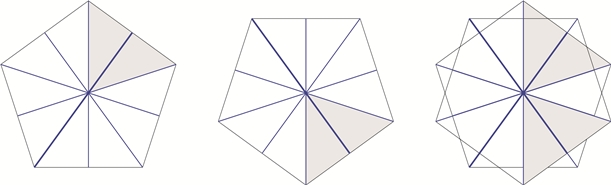
\includegraphics[width=0.7\linewidth]{pentagon_wrong.jpg}
\par
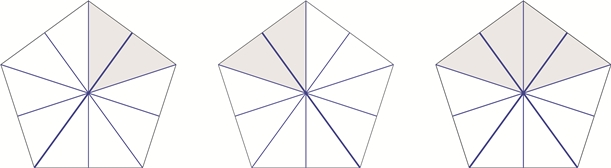
\includegraphics[width=0.7\linewidth]{pentagon_right.jpg}\\
\end{center}
The trouble however is that there are supposed to be two distinct orbits, each with K distinct elements, with 2 stabilizers. Now one stabilizer is identity, and so the other must be rotation by \emph{some} angle (the angle must actually be $\pi$, since $p$ and $p'$ are the only points in their orbit) along an axis containing the element.\\
As has been shown, one of the orbits consists of the poles corresponding to the vertices of the k-gon. (I've come back to poles since poles are what we derived the ``famous formula'' using.)
\par
The text says that the vertices \& the centres of the faces of the K-gon \emph{correspond} to the remaining poles.
\par
So essentially, the centre of faces, which in this case may even be taken to be the centre of the edges, also form an orbit such that each element has 2 stabilizers (one is identity, the other rotation by $\pi$ [effectively a reflection along the chosen axis]).\\
Now two interesting cases arise. When K is odd, say 5 for a pentagon, the poles made by opposite face/edge centre and vertex, correspond to the same axis. Yet, when the pentagon is rotated, the vertices go to the vertices, and the face/edge centres go to themselves, preserving 2 different orbits. Take a moment to realize that there aren't any other poles such that their stabilizer is of order two and they restrict the orbit of $p$ and $p'$ to $p,p'$.\\
In this case, the reflections as was shown earlier, map the pentagon to a pentagon so the orbits are preserved.\\
\begin{center}
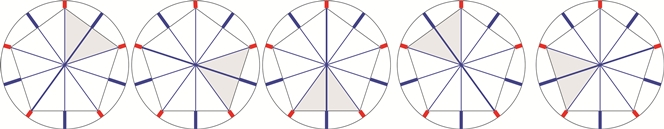
\includegraphics[width=0.7\linewidth]{pentagon_rotations.jpg}\\
\end{center}
\par
And when K is even, say 4, the poles made by opposite faces/edge centres form an axis, and those made by opposite vertices, form a different axis. And again, the poles made by the faces goto faces (under rotation by $2\pi/K$) \& correspondingly the poles made by the vertices, goto vertices. So the orbits continue to be separate!
\begin{center}
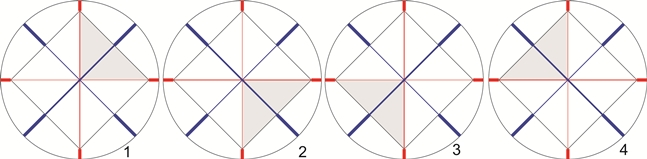
\includegraphics[width=0.5\linewidth]{square_rotations.jpg}\\
\end{center}
\par
NOTE: I did not include reflection in the analysis above since again, the reflections along both kind of axis, map the square to a square, and the orbits are thereby preserved.\\
\begin{center}
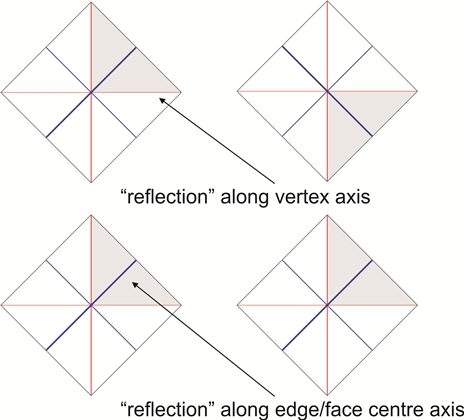
\includegraphics[width=0.4\linewidth]{square_reflections.jpg}
\end{center}
\vspace{40pt}
With that done, lets move on to the next case.\\
The arguments in the book are easy to follow. The conclusion is given as follows:
\begin{enumerate}[(a)]
\item $r_{i}=2,3,4;\,\,n_{i}=6,4,4;\,\,N=12$
\par
The poles in the orbit $O_{3}$ are the vertices of a regular tetrahedron, and G is the tetrahedral group T of its 12 rotational symmetries.
\item $r_{i}=2,3,4;\,\,n_{i}=12,8,6;\,\,N=24$
\par
The poles in the orbit $O_{3}$ are the vertices of a regular octahedron, and G is the octahedral group $O$ of its 24 rotational symmetries.
\item $r_{i}=2,3,5;\,\,n_{i}=30,20,12;\,N=60$
\par
The poles in the orbit $O_{3}$ are the vertices of a regular icosahedron, and G is the icosahedral group I of its 60 rotational symmetries.\\
\end{enumerate}
\par

In Artin the explanation for the number of symmetries for the first two shapes is probably left as an exercise.\\
However an attempt to understand the concept of ``truncated polyhedron'' seems futile without first deriving these simpler, more intuitive results.\\
\begin{enumerate}[(a)]
\item
So for a tetrahedron, we can begin the analysis by considering the rotational symmetry about its vertices. Note that the symmetrical axis about a vertex, passes through the centre of the face on the opposite side. So we will not count the rotational symmetry for the faces. So we have a $3$ fold symmetry, of which one element in the group will be identity, which will be common, so there are $2$ distinct group elements corresponding to each vertex. Also, there are $4$ vertices. So there are $2 \times 4 = 8$ non-identity elements in the group, because of symmetry of vertices (and faces). The remaining elements come from the rotation along an axis through the centre of edges, but we must be careful here as well, for each axis of symmetry passes through the centre of 2 edges. Also, the symmetry is $2$ fold, and only $1$ element is therefore non-identity. There are $6$ edges, $3$ of which share an axis, so we have $1 \times 3 = 3$ more non-identity elements in the group.\\
The total then becomes $8 + 3 + 1 \text{ (the identity element) } = 12$ and that's precisely what was expected.
\par
\item
Now the next shape is an octahedron.\\
{\bf < incomplete > }
\end{enumerate}
\vspace{20pt}
\hrule
The images of the polygons used in this document were specifically created for this purpose.\\
Rest of the images were taken from Wikipedia.
\end{document}
